\section{Results}

We applied several different classifiers with varying results. The following sections will go into details and also present the data preprocessing steps. The results presented below are based on AUC and we also added the ROC plots for each classifier.
\newline
There will be two sets of plots and results for each classifier: one computed the true positive and false positive rates comparing the class probabilities outputed by the classifier with the probabilities obtained from Alexa, the other one uses floor and ceil on the probabilities to get an exact class assignment (for example if a website has a 20\% male probability and 80\% female probability it will be assigned as 100\% female) on both classifier results and Alexa results. The results are improved.

\subsection{Preprocessing}

Initially all stop words are removed from the web pages we collected but the text goes through several other transformations.
\newline
|CountVectorizer|\footnote{\url{http://scikit-learn.org/stable/modules/generated/sklearn.feature_extraction.text.CountVectorizer.html}} converts a collection of text documents to a matrix of token counts. It was used in order to generate n-grams, limit the number of features extracted and plays a role in the process of stemming.
\newline
|TfidfTransformer|\footnote{\url{http://scikit-learn.org/stable/modules/generated/sklearn.feature_extraction.text.TfidfTransformer.html}} helps scale down the effect of the raw frequency of common words words in the corpus and adjust the weights based on how informative the features are.
\newline
|Stemming/WordNetLemmatizer|\footnote{\url{http://scikit-learn.org/stable/modules/feature_extraction.html}} refers to the process of reducing the words to their root form such that different variations of the same word do not influence the classification problem.

\subsection{Classifiers}

|SGD|\footnote{Stochastic gradient descent}\footnote{\url{http://scikit-learn.org/stable/modules/generated/sklearn.linear_model.SGDClassifier.html}} classifier refers to an iterative process of minimizing an objective function. The |loss| function is |log| which gives logistic regression, this refers to a regression model where the dependent variables are categorical.

\begin{figure}[ht!]
\centering
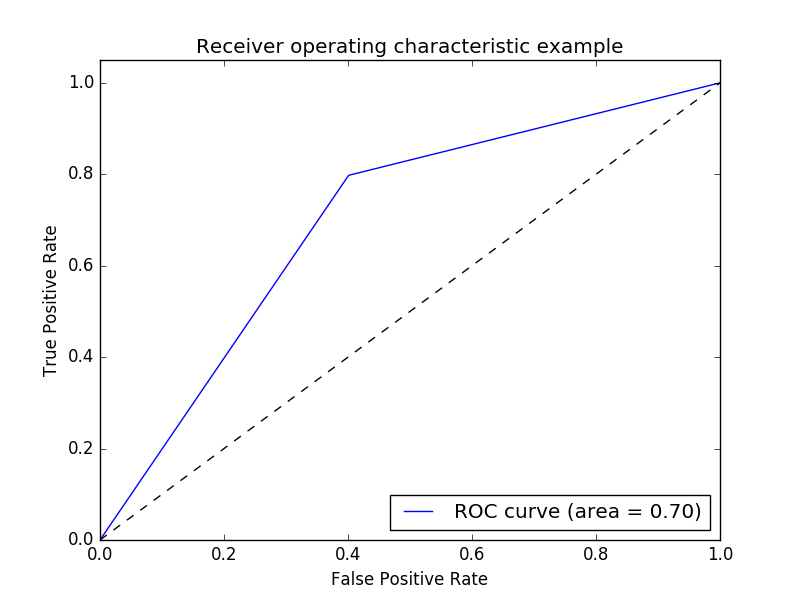
\includegraphics[width=23em]{images/out_sgdc_2.png}
\caption{ROC curve for SGD classifier}
\end{figure}

\begin{figure}[ht!]
\centering
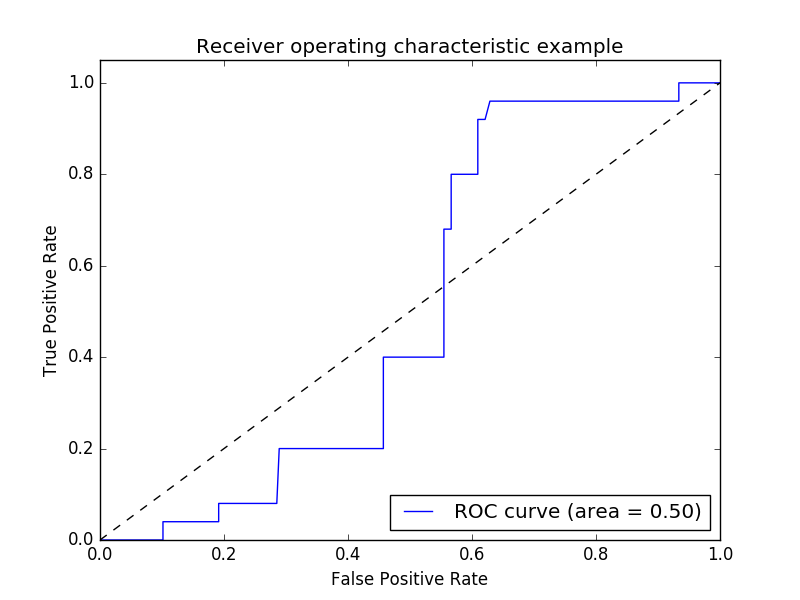
\includegraphics[width=23em]{images/out_sgd.png}
\caption{ROC curve for SGD classifier}
\end{figure}

\FloatBarrier

|NaiveBayes|\footnote{\url{http://scikit-learn.org/stable/modules/naive_bayes.html}} classifier based on Bayes' theorem in order to classify the probability of class assignment for a given input. It is fast to train with almost no parameters to adjust. It is not however a good estimator, the probabilities are not useful only hard classification results are used.

\begin{figure}[ht!]
\centering
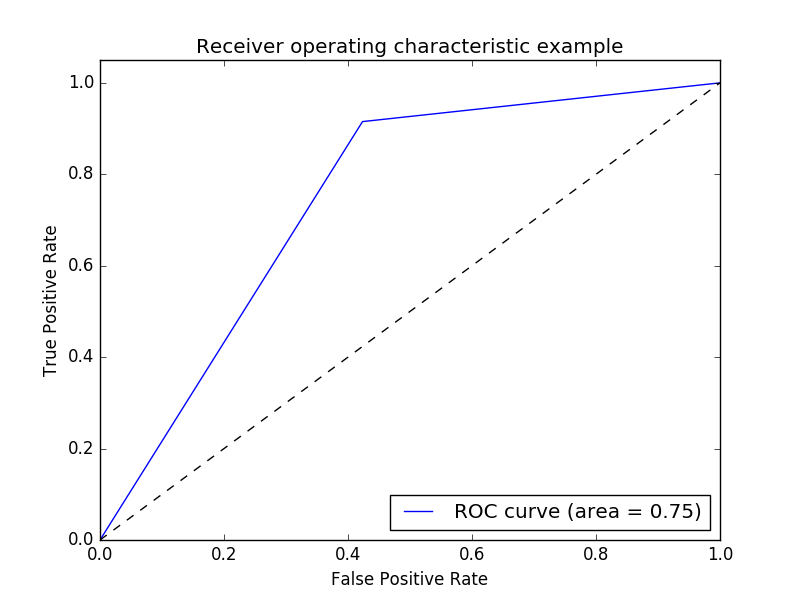
\includegraphics[width=23em]{images/out_bn.png}
\caption{ROC curve for bayes classifier}
\end{figure}

\begin{figure}[ht!]
\centering
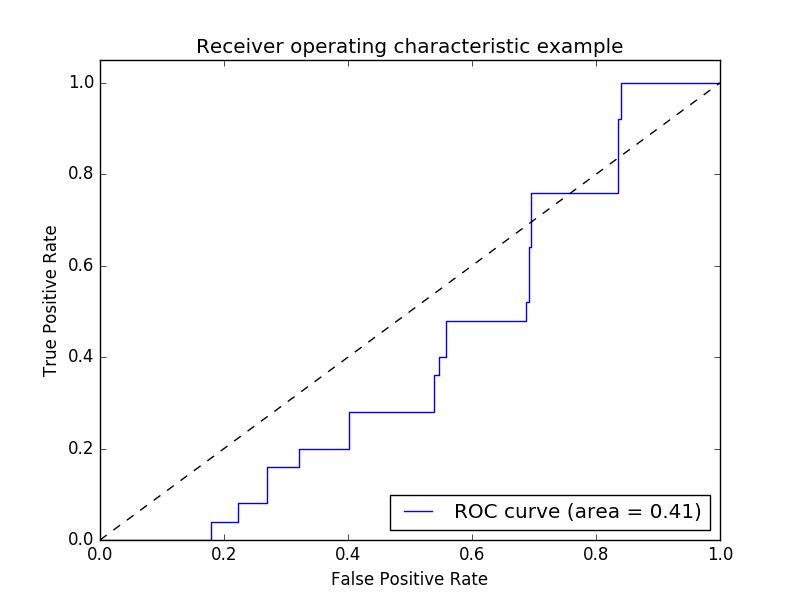
\includegraphics[width=23em]{images/out_bn2.png}
\caption{ROC curve for bayes classifier}
\end{figure}

\FloatBarrier

|RandomForest|\footnote{\url{http://scikit-learn.org/stable/modules/generated/sklearn.ensemble.RandomForestClassifier.html}} classifier based on decision trees for sub samples of the input of various sizes and with different weights. This classifier works by constructing a multitude of decision trees and associated weights at learning time, the output class is the mode of the classes or the mean prediction in case of regression.

\begin{figure}[ht!]
\centering
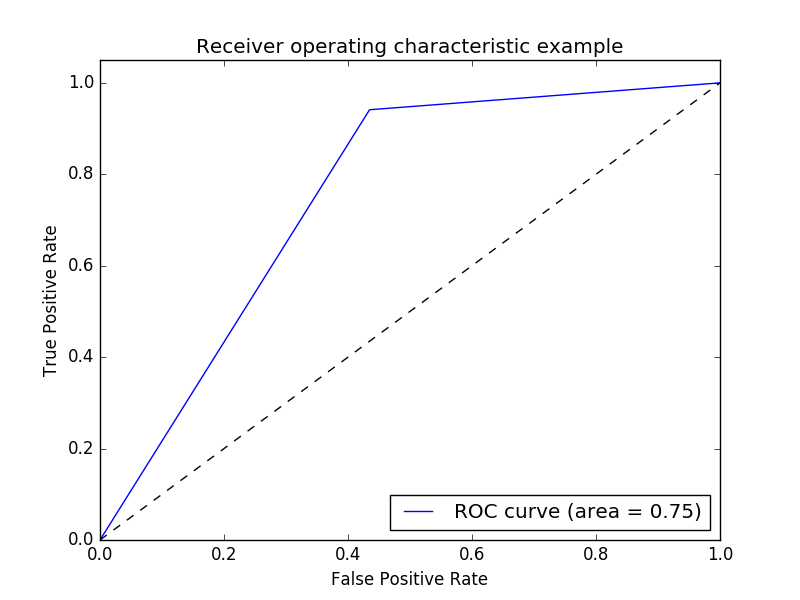
\includegraphics[width=23em]{images/out_forest_2.png}
\caption{ROC curve for random forest classifier}
\end{figure}

\begin{figure}[ht!]
\centering
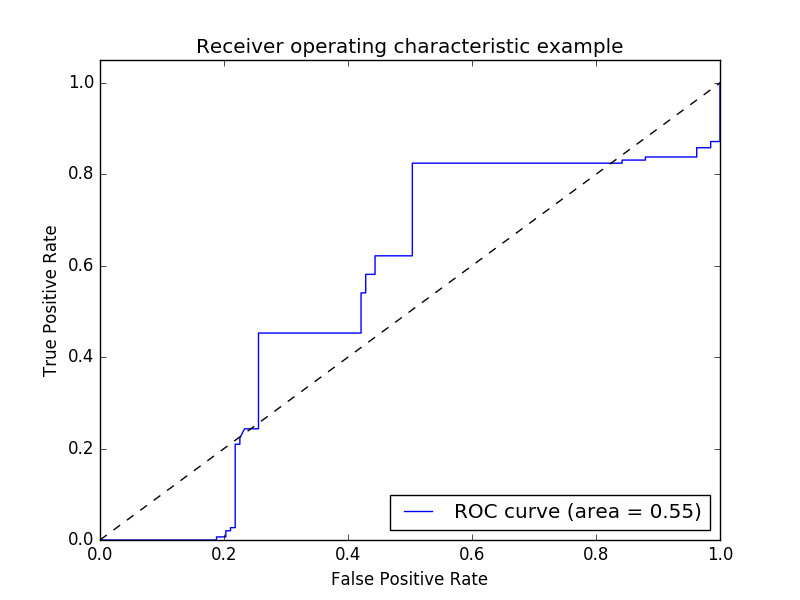
\includegraphics[width=23em]{images/out_forest.png}
\caption{ROC curve for random forest classifier}
\end{figure}

\FloatBarrier
\section{Conclusions}
As expected the Bayes clasifier has the lowest AUC results when computing probabilities but has a high degree of accuracy when used only for classification. Along with the Random Forest classifier they both scored the highest with 75\% accuracy. NaiveBayes was the easiest classifier to use, no parameter adjustment was made, the only steps involved were adjusting weights with TFIDF and stemming in preprocessing.
\newline
In our experiments, in order to get a certain degree of accuracy for gender prediction the number of websites required had to be over 200. Due to the different types of content a website might offer besides text like video or images, having less than 100 entries in the input data would give inaccurate results.
\newline
In order to train for higher results we used GridSearchCV\footnote{\url{http://scikit-learn.org/stable/modules/generated/sklearn.grid_search.GridSearchCV.html}} and optimised the text classification accuracy of our classifiers based on the dataset we collected. In our experiments this proved to also improve the ability to do website classification. To be able to train and test different models and hypothesis we actively cached as much content as possible: website text that we scraped and ratings collected from Alexa. This allowed us to eliminate the need for extra requests and speed up model training time.
\newline
The use of ngrams improved the accuracy of our classifiers, a range between [1, 3] was used for SGD classifier and [1, 2] for the other classifiers. The number of features taken into account ranges between 800 and 1000, for example one entry in our collection has 26000 words and the average is 1205 words.
